%% Workflow figure for IduEdu / Smart Cities manuscript (Figure 1).
%% Standalone TikZ -> workflow_figure.pdf, included via \includegraphics.
%% Pipeline: open urban data -> GeoDataFrame-native UrbanGraph ->
%% routing primitives (IduEdu) + ObjectNat/custom algorithms ->
%% travel-time outputs -> indicators & maps -> planning; scenario edits
%% close the loop back to the graph tables.
\documentclass[border=8pt]{standalone}
\usepackage[T1]{fontenc}
\usepackage{helvet}
\renewcommand{\familydefault}{\sfdefault}
\usepackage{tikz}
\usetikzlibrary{arrows.meta, positioning, backgrounds, fit, calc}

% ---- palette (muted, print- and colorblind-safe) ----
\definecolor{dataBd}{HTML}{475569}\definecolor{dataFl}{HTML}{EEF2F7}
\definecolor{graphBd}{HTML}{0F766E}\definecolor{graphFl}{HTML}{DFF1EE}
\definecolor{algoBd}{HTML}{7C5CBF}\definecolor{algoFl}{HTML}{F1ECFB}
\definecolor{outBd}{HTML}{2563A8}\definecolor{outFl}{HTML}{E7F0FA}
\definecolor{planBd}{HTML}{B45309}\definecolor{planFl}{HTML}{FBF0E3}
\definecolor{iduClr}{HTML}{0F766E}
\definecolor{downClr}{HTML}{B45309}
\definecolor{loopClr}{HTML}{B45309}
\definecolor{bandFl}{HTML}{F2FAF8}
\definecolor{bandBd}{HTML}{9DC9C2}

\newcommand{\hd}{\small\bfseries}

\begin{document}
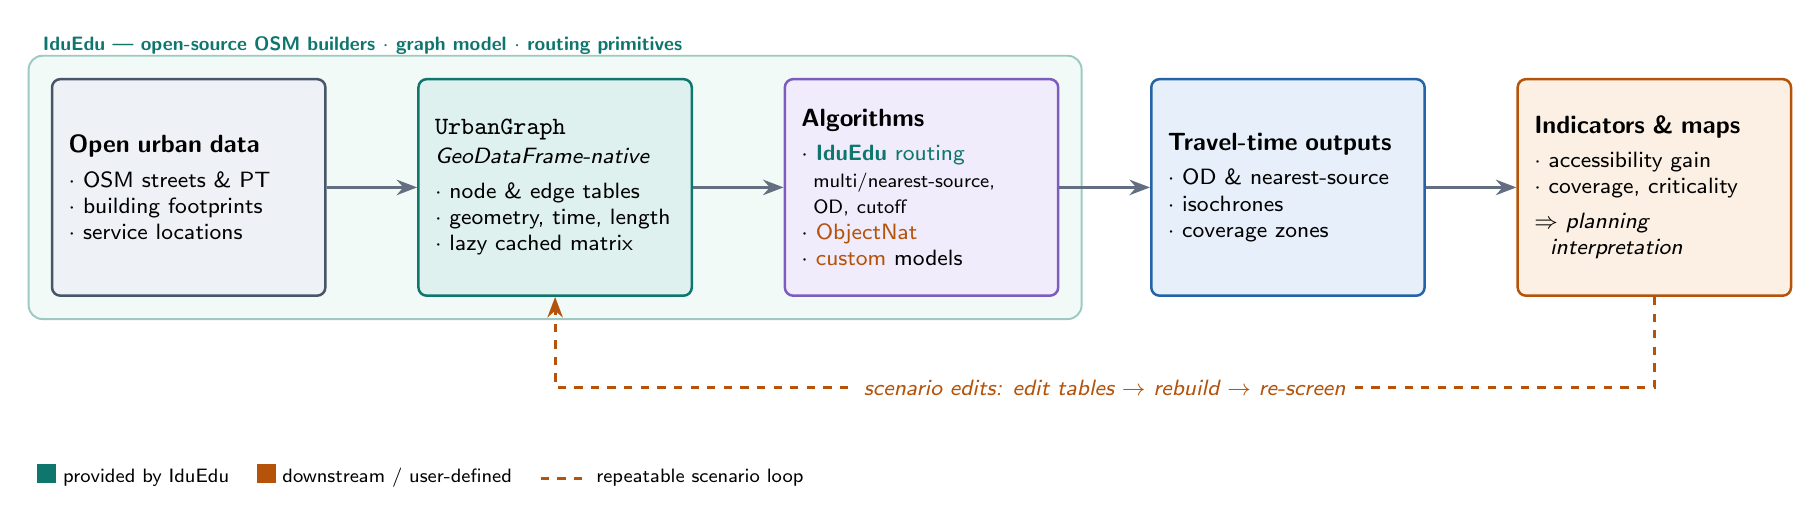
\begin{tikzpicture}[
  font=\footnotesize,
  >={Stealth[length=2.6mm]},
  stage/.style={rounded corners=3pt, draw, line width=0.9pt,
                text width=3.05cm, minimum height=2.75cm, align=left,
                inner sep=6pt, anchor=north},
  flow/.style={->, line width=1.2pt, draw=dataBd!85},
]

% ---------- pipeline stages ----------
\node[stage, draw=dataBd, fill=dataFl] (data) at (0,0)
  {{\hd Open urban data}\\[3pt]
   $\cdot$ OSM streets \& PT\\
   $\cdot$ building footprints\\
   $\cdot$ service locations};

\node[stage, draw=graphBd, fill=graphFl, right=1.15cm of data] (graph)
  {{\hd\texttt{UrbanGraph}}\\[1pt]
   {\itshape GeoDataFrame-native}\\[3pt]
   $\cdot$ node \& edge tables\\
   $\cdot$ geometry, time, length\\
   $\cdot$ lazy cached matrix};

\node[stage, draw=algoBd, fill=algoFl, right=1.15cm of graph] (algo)
  {{\hd Algorithms}\\[3pt]
   $\cdot$ \textcolor{iduClr}{\textbf{IduEdu} routing}\\
   \hspace*{1.5mm}{\scriptsize multi/nearest-source,}\\
   \hspace*{1.5mm}{\scriptsize OD, cutoff}\\
   $\cdot$ \textcolor{downClr}{ObjectNat}\\
   $\cdot$ \textcolor{downClr}{custom} models};

\node[stage, draw=outBd, fill=outFl, right=1.15cm of algo] (out)
  {{\hd Travel-time outputs}\\[3pt]
   $\cdot$ OD \& nearest-source\\
   $\cdot$ isochrones\\
   $\cdot$ coverage zones};

\node[stage, draw=planBd, fill=planFl, right=1.15cm of out] (plan)
  {{\hd Indicators \& maps}\\[3pt]
   $\cdot$ accessibility gain\\
   $\cdot$ coverage, criticality\\[3pt]
   $\Rightarrow$ {\itshape planning\\ \hspace*{2mm}interpretation}};

% ---------- forward flow ----------
\draw[flow] (data) -- (graph);
\draw[flow] (graph) -- (algo);
\draw[flow] (algo) -- (out);
\draw[flow] (out) -- (plan);

% ---------- IduEdu span band (behind data..algo) ----------
\begin{scope}[on background layer]
  \node[rounded corners=5pt, fill=bandFl, draw=bandBd, line width=0.7pt,
        fit=(data)(graph)(algo), inner sep=8pt] (band) {};
\end{scope}
\node[anchor=north west, iduClr, font=\scriptsize\bfseries]
  at ($(band.north west)+(2pt,10pt)$)
  {IduEdu — open-source OSM builders $\cdot$ graph model $\cdot$ routing primitives};

% ---------- scenario feedback loop ----------
\coordinate (pb) at (plan.south);
\coordinate (gb) at (graph.south);
\coordinate (low) at ($(gb)+(0,-1.15cm)$);
\draw[->, line width=1.1pt, dashed, draw=loopClr]
  (pb) -- ($(pb)+(0,-1.15cm)$) -- (low) -- (gb);
\node[loopClr, font=\footnotesize\itshape, fill=white, inner sep=2.5pt]
  at ($(low)!0.5!($(pb)+(0,-1.15cm)$)$)
  {scenario edits: edit tables $\rightarrow$ rebuild $\rightarrow$ re-screen};

% ---------- legend ----------
\node[anchor=north west, font=\scriptsize] at ($(band.south west)+(0,-1.7cm)$) (leg) {%
  \textcolor{iduClr}{\rule{2.4mm}{2.4mm}}~provided by IduEdu \quad
  \textcolor{downClr}{\rule{2.4mm}{2.4mm}}~downstream / user-defined \quad
  \tikz[baseline=-0.5ex]{\draw[loopClr, dashed, line width=1pt] (0,0)--(6mm,0);}~repeatable scenario loop};

\end{tikzpicture}
\end{document}
